\documentclass[a4paper]{report}
\usepackage[french]{babel}
\usepackage[utf8]{inputenc}
\usepackage[]{amsmath}
\usepackage[]{braket} % \bra, \ket etc
\usepackage{graphicx}
\usepackage{tikz}
\usepackage{subcaption} % package pour faire des subfigures
\usepackage{multirow} % package pour multirow/multicolumn
\usepackage{booktabs} % package pour top/mid/bottom rule
\usetikzlibrary{optics}
\usetikzlibrary{shapes}
\usetikzlibrary{fit}

\title{Titre}
\author{Clément Pellet-Mary}
\date\today

\begin{document}
\chapter{Lambda system}
  \section{Présentation}
  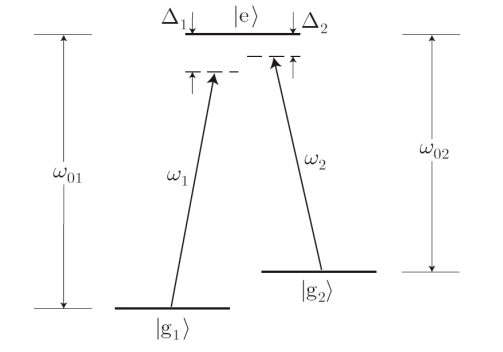
\includegraphics[width=\textwidth]{lambdasystem}
  On va considérer un couplage (sinusoïdal) uniquement entre $\ket{e}$ et $\ket{g_1}$ et entre $\ket{e}$ et $\ket{g_2}$. Le Hamiltonien du système s'écrit donc :
  \begin{equation}
  H=\hbar \begin{pmatrix}
  \omega_e & -\dfrac{\Omega_{R1}}{2}e^{-i\phi_1}e^{-i\omega_1t} & -\dfrac{\Omega_{R2}}{2}e^{-i\phi_2}e^{-i\omega_2t} \\
  -\dfrac{\Omega_{R1}}{2}e^{i\phi_1}e^{i\omega_1t} & \omega_{g1} & 0 \\
  -\dfrac{\Omega_{R2}}{2}e^{i\phi_2}e^{i\omega_2t} & 0 & \omega_{g2}
  \end{pmatrix}
  \end{equation}
  où $\phi_1$ et $\phi_2$ sont les composantes complexes des pulsations de Rabi $\Omega_{R1}$ et $\Omega_{R2}$.
  
  Dans ces conditions, on écrira un état quelconque du système à 3 niveaux sous la forme : 
  \begin{equation}
  \ket{\psi}=c_e e^{-i\omega_et} \ket{e} + c_{g1} e^{-i\omega_{g1}t} \ket{g1} + c_{g2} e^{-i\omega_{g2}t} \ket{g2}
  \end{equation}
  \subsection{Résolution dans le cas résonnant}
  En supposant que $\omega_1 = \omega_e - \omega_{g1}$ et $\omega_2 = \omega_e - \omega_{g2}$, on déduit de Schrödinger : 

  \begin{align}
  \label{schro_resonnant}
  \dot{c_e}&=\dfrac{i}{2}(\Omega_{R1}e^{-i\phi_1}c_{g1}+\Omega_{R2}e^{-i\phi_2}c_{g2})\\
  \dot{c_{g1}}&=\dfrac{i}{2}\Omega_{R1}e^{i\phi_1}c_e \\
  \dot{c_{g2}}&=\dfrac{i}{2}\Omega_{R2}e^{i\phi_2}c_e 
  \end{align}
  
\section{Dark State}
On va se placer dans le cas résonnant, et on va considérer un état initialement dans une superposition des états fondamentaux : 
\begin{equation}
\label{psi0}
\ket{\psi}(t=0)=\cos\dfrac{\theta}{2} \ket{g1} + \sin\dfrac{\theta}{2} e^{i \psi}\ket{g2}
\end{equation}

Alors, en résolvant les équations \ref{schro_resonnant}, on trouve que :
\begin{equation}
c_e(t)=\dfrac{i \sin (\Omega t /2)}{\Omega}\left[\Omega_{R1}e^{-i\phi_1} \cos\dfrac{\theta}{2} + \Omega_{R2}e^{-i(\phi_2+\psi)} \sin\dfrac{\theta}{2} \right]
\end{equation}
où $\Omega = \sqrt{\Omega_{R1}^2+\Omega_{R2}^2}$. $c_{g1}$ et $c_{g2}$ peuvent se calculer mais c'est chiant.

On voit que pour certaines valeurs de $\theta$ et certains paramètres de couplage, tu peux annuler $c_e$, et donc créer un dark state, un état fondamental qui n'est pas excité par des champs résonnants. La condition c'est que :
\begin{equation}
\dfrac{\sin (\theta/2)}{\cos (\theta/2)} = \tan (\theta/2) = - \dfrac{\Omega_{R1}}{\Omega_{R2}} e^{-i(\phi_1-\phi_2-\psi)}
\end{equation}

ce qui te permet d'écrire, en remplaçant dans \ref{psi0} que le dark state généralisé s'écrit comme : 
\begin{equation}
\ket{\psi(t)}=\dfrac{\Omega_{R2}(t)e^{-i\phi_2}\ket{g1}+\Omega_{R1}(t)e^{-i\phi_1}\ket{g2}}{\sqrt{\Omega_{R1}^2+\Omega_{R2}^2}}
\end{equation}

Dans le cas où tu peux négliger les composantes complexes, tu vois qu'une façon de créer un dark state c'est de partir de $\ket{g1}$, avec $\Omega_{R2}$ allumé, mais $\Omega_{R1}$ éteint, puis d'allumer progressivement (adiabatiquement) $\Omega_{R1}$. (D'ailleurs ça marche même si tu ne négliges pas les composantes complexes).

Ca s'appelle du STImulated Raman Adiabatic Passage (STIRAP), et a priori, "lentement" ici c'est par rapport aux fréquences de Rabi, puisqu'il faut que les populations ait le temps de s'équilibrer. Bon c'est un peu bizarre vu que c'est justement la pulsation de Rabi que tu modifies, mais je le comprend comme : si tu veux atteindre un couplage $\Omega_R$, tu dois le faire dans un temps grand devant $1/\Omega_R$. Ca peut permettre de passer de $\ket{g1}$ à $\ket{g2}$ de façon plus certaine que par une pulse Rabi $\pi$

\section{Electromagnetically Induced Transparency (EIT)}

La suite au prochain épisode
 
  \end{document}	
  
  